\documentclass[11pt,a4paper]{article}

\usepackage[utf8]{inputenc}
\usepackage[T1]{fontenc}
\usepackage{geometry}
\usepackage{graphicx}
\usepackage[hidelinks]{hyperref}

\geometry{margin=2.5cm}

\begin{document}

%======================
% Cover page
%======================
\begin{titlepage}
    \centering

    \begin{minipage}{0.45\textwidth}
        \centering
        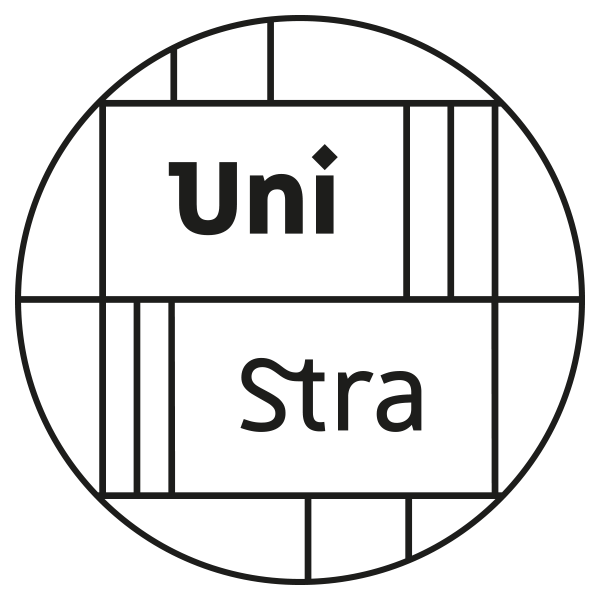
\includegraphics[width=0.55\textwidth]{logo_unistra.png}
    \end{minipage}
    \hfill
    \begin{minipage}{0.45\textwidth}
        \centering
        
\includegraphics[width=0.55\textwidth]{logo_quantum_bluff.png}
    \end{minipage}

    \vspace{2.5cm}

    {\Huge \textbf{Quantum Bluff}\par}
    \vspace{0.4cm}
    {\Large Final Project Report\par}

    \vspace{1cm}
    {\large University of Strasbourg -- L3 Computer Science\par}

    \vspace{1.5cm}
    {\large
    Project Manager: Omar\\
    Team: Linda, Massi, Abdoulaye, Soheil, Mohamed, Azra, Yigit
    \par}

    \vfill
    {\large 2026\par}
\end{titlepage}

%======================
% Table of contents
%======================
\tableofcontents
\newpage

%======================
% Report structure
%======================

\section{Introduction}

\subsection{Context and Objectives}

Quantum Bluff was developed as part of the final third-year Bachelor's degree project (L3 Computer Science, French academic system) at the University of Strasbourg. The objective of the project was to design and implement a complete real-time multiplayer gaming platform combining advanced software engineering concepts, distributed systems, web technologies and team-based project management within a collaborative development environment.

The initial goal of the project was to create a Texas Hold'em poker platform playable both against artificial intelligence bots with multiple difficulty levels and in multiplayer mode through online public or private tables. Beyond gameplay implementation, the project also aimed to address several technical challenges such as real-time synchronization, distributed communication, secure transaction management, low-latency multiplayer interactions and horizontal scalability through Redis-backed synchronization systems.

Another important objective was to reproduce a professional software engineering workflow inside an academic project. The team therefore worked on requirement analysis, software architecture, testing, observability, deployment, continuous integration and collaborative development practices while adapting the project organization according to evolving technical and functional requirements.

Special attention was also given to security and reliability aspects through the integration of JWT authentication, two-factor authentication (2FA), anti-cheat mechanisms, API rate limiting, idempotent transaction handling and schema-based validation on critical API paths.

\subsection{Project Overview}

Quantum Bluff progressively evolved from a simple poker application into a complete multiplayer casino platform integrating several independent yet interconnected systems. The final platform includes Texas Hold'em Poker, Blackjack, Roulette and Slot Machine game modes, together with tournaments, leaderboards, hidden betting systems, XP progression, badges, profile customization and multilingual support.

The application is based on a monorepo architecture composed of a React frontend and a Node.js / Express backend communicating in real time through Socket.IO. Data persistence is managed using PostgreSQL and Prisma, while Redis is used for distributed synchronization, rate limiting, action logging and multi-instance Socket.IO communication.

The platform also integrates advanced systems such as client-side poker equity estimation, server-side pricing and resolution for hidden bets, AI bots, social systems including friends and in-game loans, tournament winner betting systems, interactive tutorials and automated runtime recovery mechanisms.

From a software engineering perspective, the project includes structured logging, Prometheus metrics, OpenTelemetry observability tools, Jest and Vitest testing suites, Playwright end-to-end testing, GitLab continuous integration workflows and multi-platform deployment support through Electron and Capacitor for desktop and mobile environments.

Throughout the project, particular attention was given to modularity, maintainability, clear module boundaries and collaborative development practices in order to simulate conditions close to a professional software engineering environment.
\newpage
\section{Project Evolution}

\subsection{Initial Specifications}

At the beginning of the project, Quantum Bluff was initially designed as a focused Texas Hold'em poker platform combining both single-player and multiplayer functionalities. The early scope of the project targeted a system where users could either play against artificial intelligence bots with multiple difficulty levels or join multiplayer poker tables through public and private rooms.

Early functional requirements included configurable small blind and big blind values, minimum balance conditions for joining tables, real-time multiplayer synchronization and a probability HUD capable of displaying estimated winning probabilities and hand statistics during gameplay. Another important feature planned from the beginning was the hidden betting system, allowing players to place side bets on game outcomes and poker events.

From a technical perspective, the project was designed around a monorepo architecture with a React frontend and a Node.js / Express backend communicating through Socket.IO for real-time interactions. PostgreSQL and Prisma were selected for persistence management, while Redis was adopted early for distributed synchronization, rate limiting and Socket.IO multi-instance communication.

The project organization initially followed a V-Model approach with separated phases for requirement analysis, specification validation, implementation and testing.

\subsection{Evolution of the Requirements}

As development progressed, the scope of the project evolved significantly beyond the original poker platform. After several weeks of development, it became clear that a strict V-Model organization limited the integration of iterative improvements and new gameplay ideas. The project workflow was therefore progressively adapted toward a more flexible and iterative organization inspired by agile development practices, using prioritized task management, short development cycles and continuous feature validation within the team.

This transition allowed the project to continuously evolve according to technical opportunities, gameplay improvements and user experience objectives. Several new functionalities and systems were progressively integrated into the platform.

Additional casino games such as Blackjack, Roulette and Slot Machine systems were developed and integrated into the shared platform ecosystem. The multiplayer architecture was also extended with tournament systems, tournament winner betting systems and advanced real-time synchronization mechanisms.

The platform furthermore evolved toward a more complete social and progression-oriented ecosystem through the addition of XP progression, badges, leaderboards and multilingual support using i18n. The scope also expanded toward social and identity features, including a friends system with invitations and presence management, configurable in-game loans between players with interest and repayment mechanisms linked to game outcomes, and profile customization systems with server-managed avatars.

From an engineering perspective, the architecture also became considerably more advanced during development. Redis integration was expanded for distributed synchronization and runtime management, while observability systems based on structured logging, Prometheus metrics and OpenTelemetry were progressively integrated. Security mechanisms were reinforced through JWT authentication, 2FA integration, anti-cheat systems, API rate limiting and idempotent transaction validation.

The project also expanded beyond a traditional web application through Electron and Capacitor integration in order to support desktop and mobile deployment environments.

\subsection{Final Delivered Product}

The final delivered version of Quantum Bluff is a complete multiplayer casino and gaming platform integrating several interconnected systems inside a unified architecture.

The platform includes Texas Hold'em Poker with multiplayer and AI bot modes, Blackjack, Roulette and Slot Machine systems, tournament management, hidden betting markets, progression mechanics and social interaction features. Real-time communication between players is handled through Socket.IO, while PostgreSQL, Prisma and Redis ensure persistent data management and distributed synchronization.

From a software engineering perspective, the final platform integrates observability tools, automated testing systems, GitLab continuous integration workflows and multi-platform deployment support through Electron and Capacitor.

Overall, the project evolved from a relatively focused multiplayer poker application into a substantial full-stack distributed platform exposing the team to many practices commonly encountered in professional software development environments.
\newpage
\section{Project Management}

\subsection{Initial V-Model Organization}

At the beginning of the project, the team adopted a V-Model organization in order to structure the development process through clearly separated phases. The project first started with requirement gathering sessions, benchmarking activities and brainstorming meetings aimed at identifying the expected functionalities, technical constraints and user experience objectives of the platform.

The initial management approach focused on defining the specifications before implementation. Functional requirements, gameplay systems and technical objectives were progressively validated during regular team meetings. A specification document and an initial Gantt planning were produced in order to organize the workload and establish development priorities for the different project phases.

This methodology was initially chosen because it provided a clear framework for coordinating a relatively large team and reducing organizational ambiguity during the early stages of development.

\subsection{Transition to a Waterfall Approach}

As development progressed, the project rapidly expanded beyond its initial scope. The integration of new gameplay systems, social features and technical improvements made the original V-Model organization increasingly difficult to maintain within the project's time constraints.

The team therefore progressively transitioned toward a more flexible development workflow inspired by iterative and incremental approaches. Instead of strictly separating specification and implementation phases, development became more continuous, with regular feature additions, progressive refinements and direct integration of feedback during implementation.

Task management evolved toward prioritized feature lists and shorter development cycles focused on delivering functional modules incrementally. This transition allowed the team to adapt more efficiently to new technical challenges, gameplay ideas and evolving project objectives while maintaining overall project coherence.

\subsection{Planning, Coordination and Reporting}

Project coordination was organized through regular meetings held approximately twice per week. These meetings were used to monitor development progress, validate technical decisions, identify blocking issues and redistribute tasks according to the current priorities of the project.

Task distribution evolved dynamically throughout development depending on technical complexity, feature dependencies and team availability. Communication between frontend, backend and infrastructure-related tasks was particularly important because of the real-time multiplayer nature of the platform.

Development progress was monitored through shared reporting documents, internal technical documentation and continuous validation sessions. Particular attention was given to bug tracking, feature validation and synchronization between the different modules of the platform in order to reduce integration issues during the later stages of development.

\subsection{Management of Technical and Human Challenges}

The project introduced several technical challenges related to real-time multiplayer synchronization, distributed state management, database consistency and large-scale feature integration. The progressive increase in project scope also required continuous architectural adjustments and improved coordination between different technical modules.

From an organizational perspective, managing a large collaborative academic project over several months required continuous communication and adaptation. Workload balancing, synchronization between contributors and maintaining development consistency became important aspects of the management process.

To address these challenges, the project organization progressively evolved toward more iterative validation practices, continuous communication and flexible task redistribution. Internal technical documentation, reporting sessions and collaborative debugging phases played an important role in maintaining project stability and ensuring that all major functionalities could be successfully integrated into the final platform.
\newpage
\section{Development Tools and Technologies}
\subsection{Frontend and Backend Technologies}
\subsection{Database and Infrastructure Tools}
\subsection{Version Control and Collaboration Tools}
\subsection{Testing and Deployment Tools}
\newpage
\section{Use of Artificial Intelligence}
\subsection{AI-Assisted Development}
\subsection{Code Generation and Debugging Assistance}
\subsection{Documentation and Productivity Support}
\subsection{Limits and Verification of AI Outputs}
\newpage
\section{Platform Functionalities}
\subsection{Poker and Tournament System}
\subsection{Hidden Bets and Probability Features}
\subsection{Casino Games and AI Bots}
\subsection{Rewards, Banking and Transactions}
\subsection{Web, Desktop and Mobile Versions}
\newpage
\section{System Architecture}
\subsection{Backend, Frontend and Database}
\subsection{Real-Time Communication}
\subsection{Redis and Distributed Infrastructure}
\subsection{Deployment and CI/CD Pipeline}
\newpage
\section{Security, Testing and Stability}
\subsection{Authentication and Anti-Cheat}
\subsection{Testing and Debugging}
\subsection{Performance and Stability Improvements}
\newpage
\section{Technical Challenges}
\subsection{Real-Time Synchronization}
\subsection{Infrastructure and Scalability}
\subsection{Implemented Solutions}
\newpage
\section{Individual Contributions}
\subsection{Omar -- Project Management and System Architecture}

As project manager, I supervised both the organizational and technical aspects of Quantum Bluff throughout the entire project lifecycle. At the beginning of the project, I structured the work using a V-Model approach, starting with requirement gathering, benchmarking and discussions with end users in order to define the platform objectives and expected functionalities. I was responsible for the MOA side of the project, including brainstorming sessions, specification validation, the writing of the requirements document and the creation of the project Gantt chart. To better organize the technical implementation, I also appointed a technical lead responsible for coordinating the MOE side of the project.

Initially, Quantum Bluff was planned as a Texas Hold'em poker platform with multiplayer support, AI bots, hidden bets and probability calculations. However, after several weeks of development, I realized that a strict V-Model approach limited the integration of new ideas and continuous improvements. I therefore reorganized the project around a more agile workflow inspired by Scrum methodologies using Jira, epics, user stories, sprints and backlog prioritization based on feature value and project objectives.

This transition allowed the project scope to expand significantly with the integration of additional systems such as Blackjack, Roulette, Slot Machine, tournaments, leaderboards, XP progression, badges, profile customization, multilingual support with i18n and an interactive tutorial system. I also supervised the global software architecture, including the Redis distributed layer, the monorepo organization, the real-time multiplayer infrastructure and the automated deployment pipeline. Throughout the project, I coordinated meetings, validated technical decisions, monitored bug fixing sessions and ensured communication between all team members.
\subsection{Mohamed -- Backend and Multiplayer Logic}
\subsection{Azra -- Frontend and User Experience}
\subsection{Linda -- Testing and Validation}
\subsection{Massi -- Infrastructure and Integration}
\subsection{Abdoulaye -- Backend Features and Database}
\subsection{Soheil -- Frontend Features}
\subsection{Yigit -- Debugging and Quality Assurance}

\section{Limitations and Future Work}
\subsection{Current Limitations}
\subsection{Future Improvements}

\section{Conclusion}

\appendix

\section{Appendices}
\subsection{Architecture Diagrams}
\subsection{Database Schema}
\subsection{Platform Screenshots}

\end{document}